\chapter{Analysis}
\section{Defining a problem}
The company is a camera auction website that allows the user to either sell or buy camera equipment. The current issue is whilst current auction websites exist that allow the user to sell an item to the highest bidder, none of them provide an experience that supports a person selling camera gear. Items such as how much the camera should be priced at can be difficult for a seller and currently there is no easy solution for people who want to sell. It can lead to devices being priced too high and thus never selling or cameras that are priced too low and so the owner misses out on what the camera is worth. As well as this, people who are looking to buy camera gear currently struggle with finding out the information of a particular camera and whether it will meet their own personal needs for a device.
The website is required to be easy to use for both buying and selling and must assist the user so that they can buy or sell the camera equipment they want easily. In order to solve the problems, program will allow the user to enter the camera that they are selling and get a price estimate for what previous cameras have hold for. This will help the user to see where they should be listing their camera in order to get a sale at the best price. In order to assist the buyer, the website will display information on the camera, such as megapixels and year released, to enable the buyer to see if the camera will meet their requirements for their specific circumstances.

\section{Stakeholders}
\subsection{Stakeholder 1: Someone selling their camera for the first time, John Smith}
This will be someone who has been doing photography for a while and has decided that they want to sell their camera. I will be asking them questions on their reasons for upgrading and what their current problems are with existing solutions. This will allow me to decide what features are best to be implemented with a seller in mind. As features are added to the platform, I will be able to check in with John in order to say whether the feature is both working and improves their experience when on the platform.
\subsection{Stakeholder 2: Someone looking to buy a camera for specific needs, Phil Martin}
This stakeholder will be looking to buy a camera, not necessarily for the first time although that is acceptable. I will ask them about why they want to buy a camera and what needs they have for such a device. By further asking them questions on what difficulties they have found with current buying solutions it will allow me to gauge what is important when buying a camera and how best my program can ease the stresses and confusion behind it. By checking in with Phil as the project progresses, it will help to ensure that the new features added still fit in a balance of supporting both the buyer and the seller. This ensures that overall, both parties get a collection of new features.
{Why the program is suited to computational methods}
This problem lends itself to a computational solution as it reduces the complexity of a real-world auction. By removing various elements of an auction, such as a physical human to lead proceedings, it creates a simpler solution not only for the user but a simpler solution to program. A computational solution is also required in order to create items such as the camera information area as there would be a large amount of information for every camera, and it would be unrealistic for a person in a conventional auction to know every detail of the camera that they are bidding on. A computer would also be required in order to produce a realistic estimate for what the camera will sell for based on sold listings.

\section{Computational methods the program lends itself to}
\subsection{Thinking abstractly}
The program will create a simplified experience of a real-life auction. Regular features of bidding and auctions lasting only a set amount of time will be kept. However, items such as bidding only being open for a small amount of time will be removed as users will be able to bid on items at any point throughout the time the item is listed.
\subsection{Thinking ahead}
The program will require data from the user for various aspects. In the user login or sign-up system for example, the program will require; a username, which must be unique, a password of a suitable length. If the user is thinking of searching for a listing, then the website will require the name of the camera from a search box field on the page. Creating an actual listing on the page will require the most amount of information from the user. This is due to them having to specify what camera they are selling and a price they want to start the bidding at as well as having to add descriptions of the camera and the quality of the item.  Data also has to be collected in order for the camera information to be displayed. 
\subsection{Decomposition}
The program has multiple functions that the user can use from listing an item to searching for a new piece of gear. This therefore means that when developing, the solution can be broken down into smaller problems that can be developed separately. Beyond this, each section can be broken down into smaller stages when developing. For example, someone searching the listings for a specific camera will be decomposed as: \begin{enumerate}
    \item User enters the name of the camera they want into the search box
    \item The field is read, and the database is searched for that item
    \item Return the various listings in a table 
\end{enumerate}

\subsection{Thinking procedurally}
With the development of the program, it can be broken down into small sections by treating each webpage as its own separate section part of the development. The program will utilise different webpages during the user’s experience. For example, the development of the sign-up page can be tackled separately to the search page. Within the development of each page, the programming can be decomposed with one section being the HTML code that has to be written in order to create the webpage and the other section being the PHP code behind the page. Elements such as a user logging into the site can be treated procedurally as each separate entering of data can be treated separately and each query that must be sent to the SQL server.
\subsection{Thinking logically}
One aspect of the program where the program with have to branch depending on a decision is the sign-up point. The username and email that the user enters will have to be checked against the database in order to ensure that someone with the same username or email has not signed up before. This will require the program to branch as if the details are unique, the user will be allowed to enter the site else the program will have to send the user back to the landing page in order to try again. The program will use looping when it comes to displaying the relevant listings after a search has been placed. The program will have to loop through the results of the SQL database query in order to output the findings in a table for the user to interact with. 
\subsection{Thinking concurrently}
Within the program, one of the aspects that can be solved concurrently is the removing of the listing at the end and the charging of the seller. When the listing is finished at the end of the time period, the bidding will need to be closed. At the same time that this happens, the site will need to charge the highest bidder’s card with the amount that they have bid for the item which will finalise the auction. Another function of the program that would suit being solved concurrently is the updating of the recommended pricing for that specific camera that has solved. This can happen at the same time as the listing closes in order to ensure that the information isn’t lost once a sold listing is removed from the site. It also ensures that the program will always give an as up to date recommendation as possible. 

\section{Research}
\subsection{Existing solution: eBay \parencite{ebay1}}
eBay is an auction website that allows the user to browse or list items on the platform. The website isn’t specifically built for the buying and selling of cameras and does allow for auction style buying and selling of products. During the process, the user has control over how much they want to start the bidding at and how long they want to allow the auction to run.
\begin{figure}[H]
    \centering
    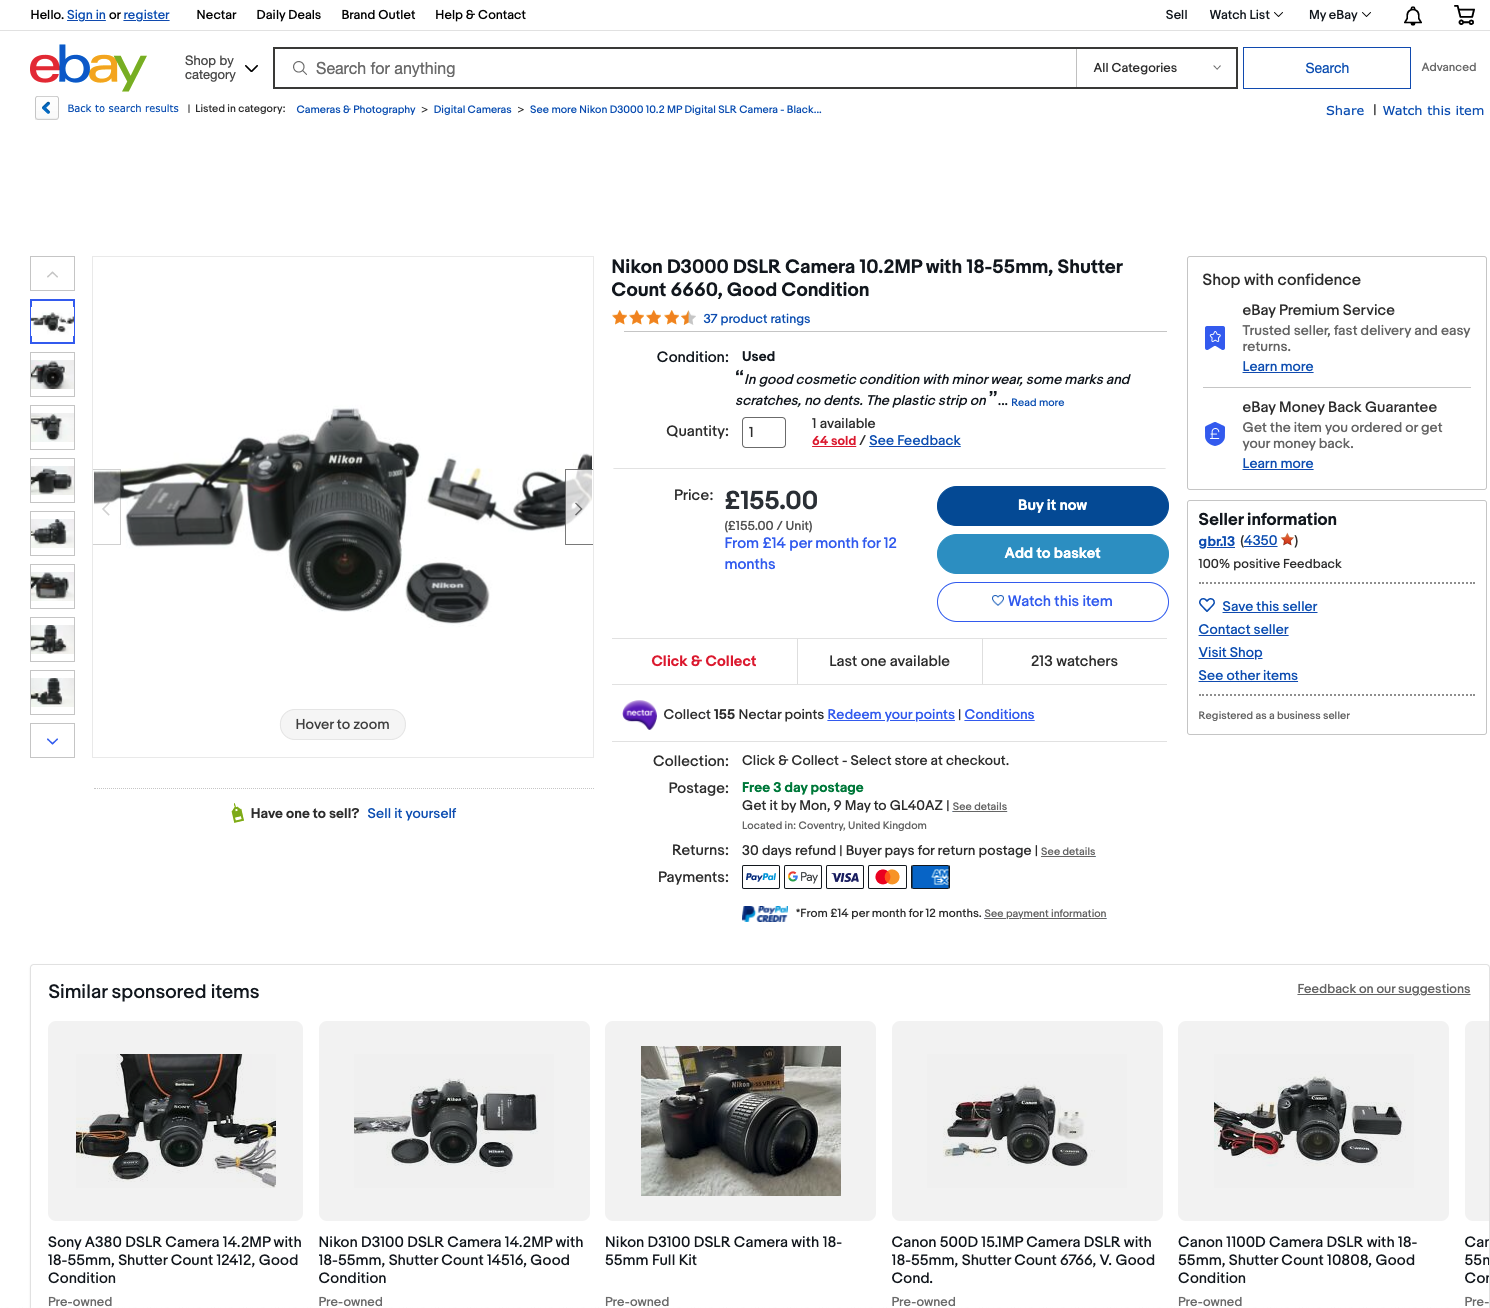
\includegraphics[scale=0.3]{ch1_analysis/ebay_listing.png}
    \caption{eBay auction listing}
    \label{fig:ch1_ebay}
\end{figure}
\subsubsection{Advantages}
One advantage of the program is that it quickly allows the user to create a listing. Within just a few clicks from the start page, the user can have an item up for sale and available for anyone to bid on. This reduces the complexity for someone who is looking to sell an item on the site. Another advantage is that similar listings are sold on the site. This enables the user to browse various other listings to see which ones matches the qualities that are needed both in device specifications but also the condition of the item.
\subsubsection{Disadvantages}
eBay is not specifically built with the buying and selling of photography gear in mind. One issue that the user might face when trying to sell is that pricing the camera can be difficult since there is no recommendation to how the user should price the camera, this therefore means that sales can be difficult. Another disadvantage of the site is that there isn’t any information for the user to browse when searching for a camera in order to see if the device will have the right specifications for the intended use case.
\subsubsection{Features to include}
One feature to take away from eBay would be the auction style system that it uses which allows the user to set the duration of the auction. This means that products that might never actually sell are not on the site forever taking up space and slowing down a buyer. Another feature to take away is the minimum buyout feature on the platform. This means that the item cannot sell for a ridiculously low price which also ensures that the seller gets a fair price for the camera. 

\subsection{Existing solution: MPB \parencite{mpb}}
MPB is a site that is dedicated to selling second hand camera gear. The site allows the user to search and browse for a camera that they want. Cameras are sorted by the make and model and are rated, from faulty to like new, on the condition of the camera. Along with this, the user can see what will come with the purchase of the camera, such as whether it includes a charger or strap.
\begin{figure}[H]
    \centering
    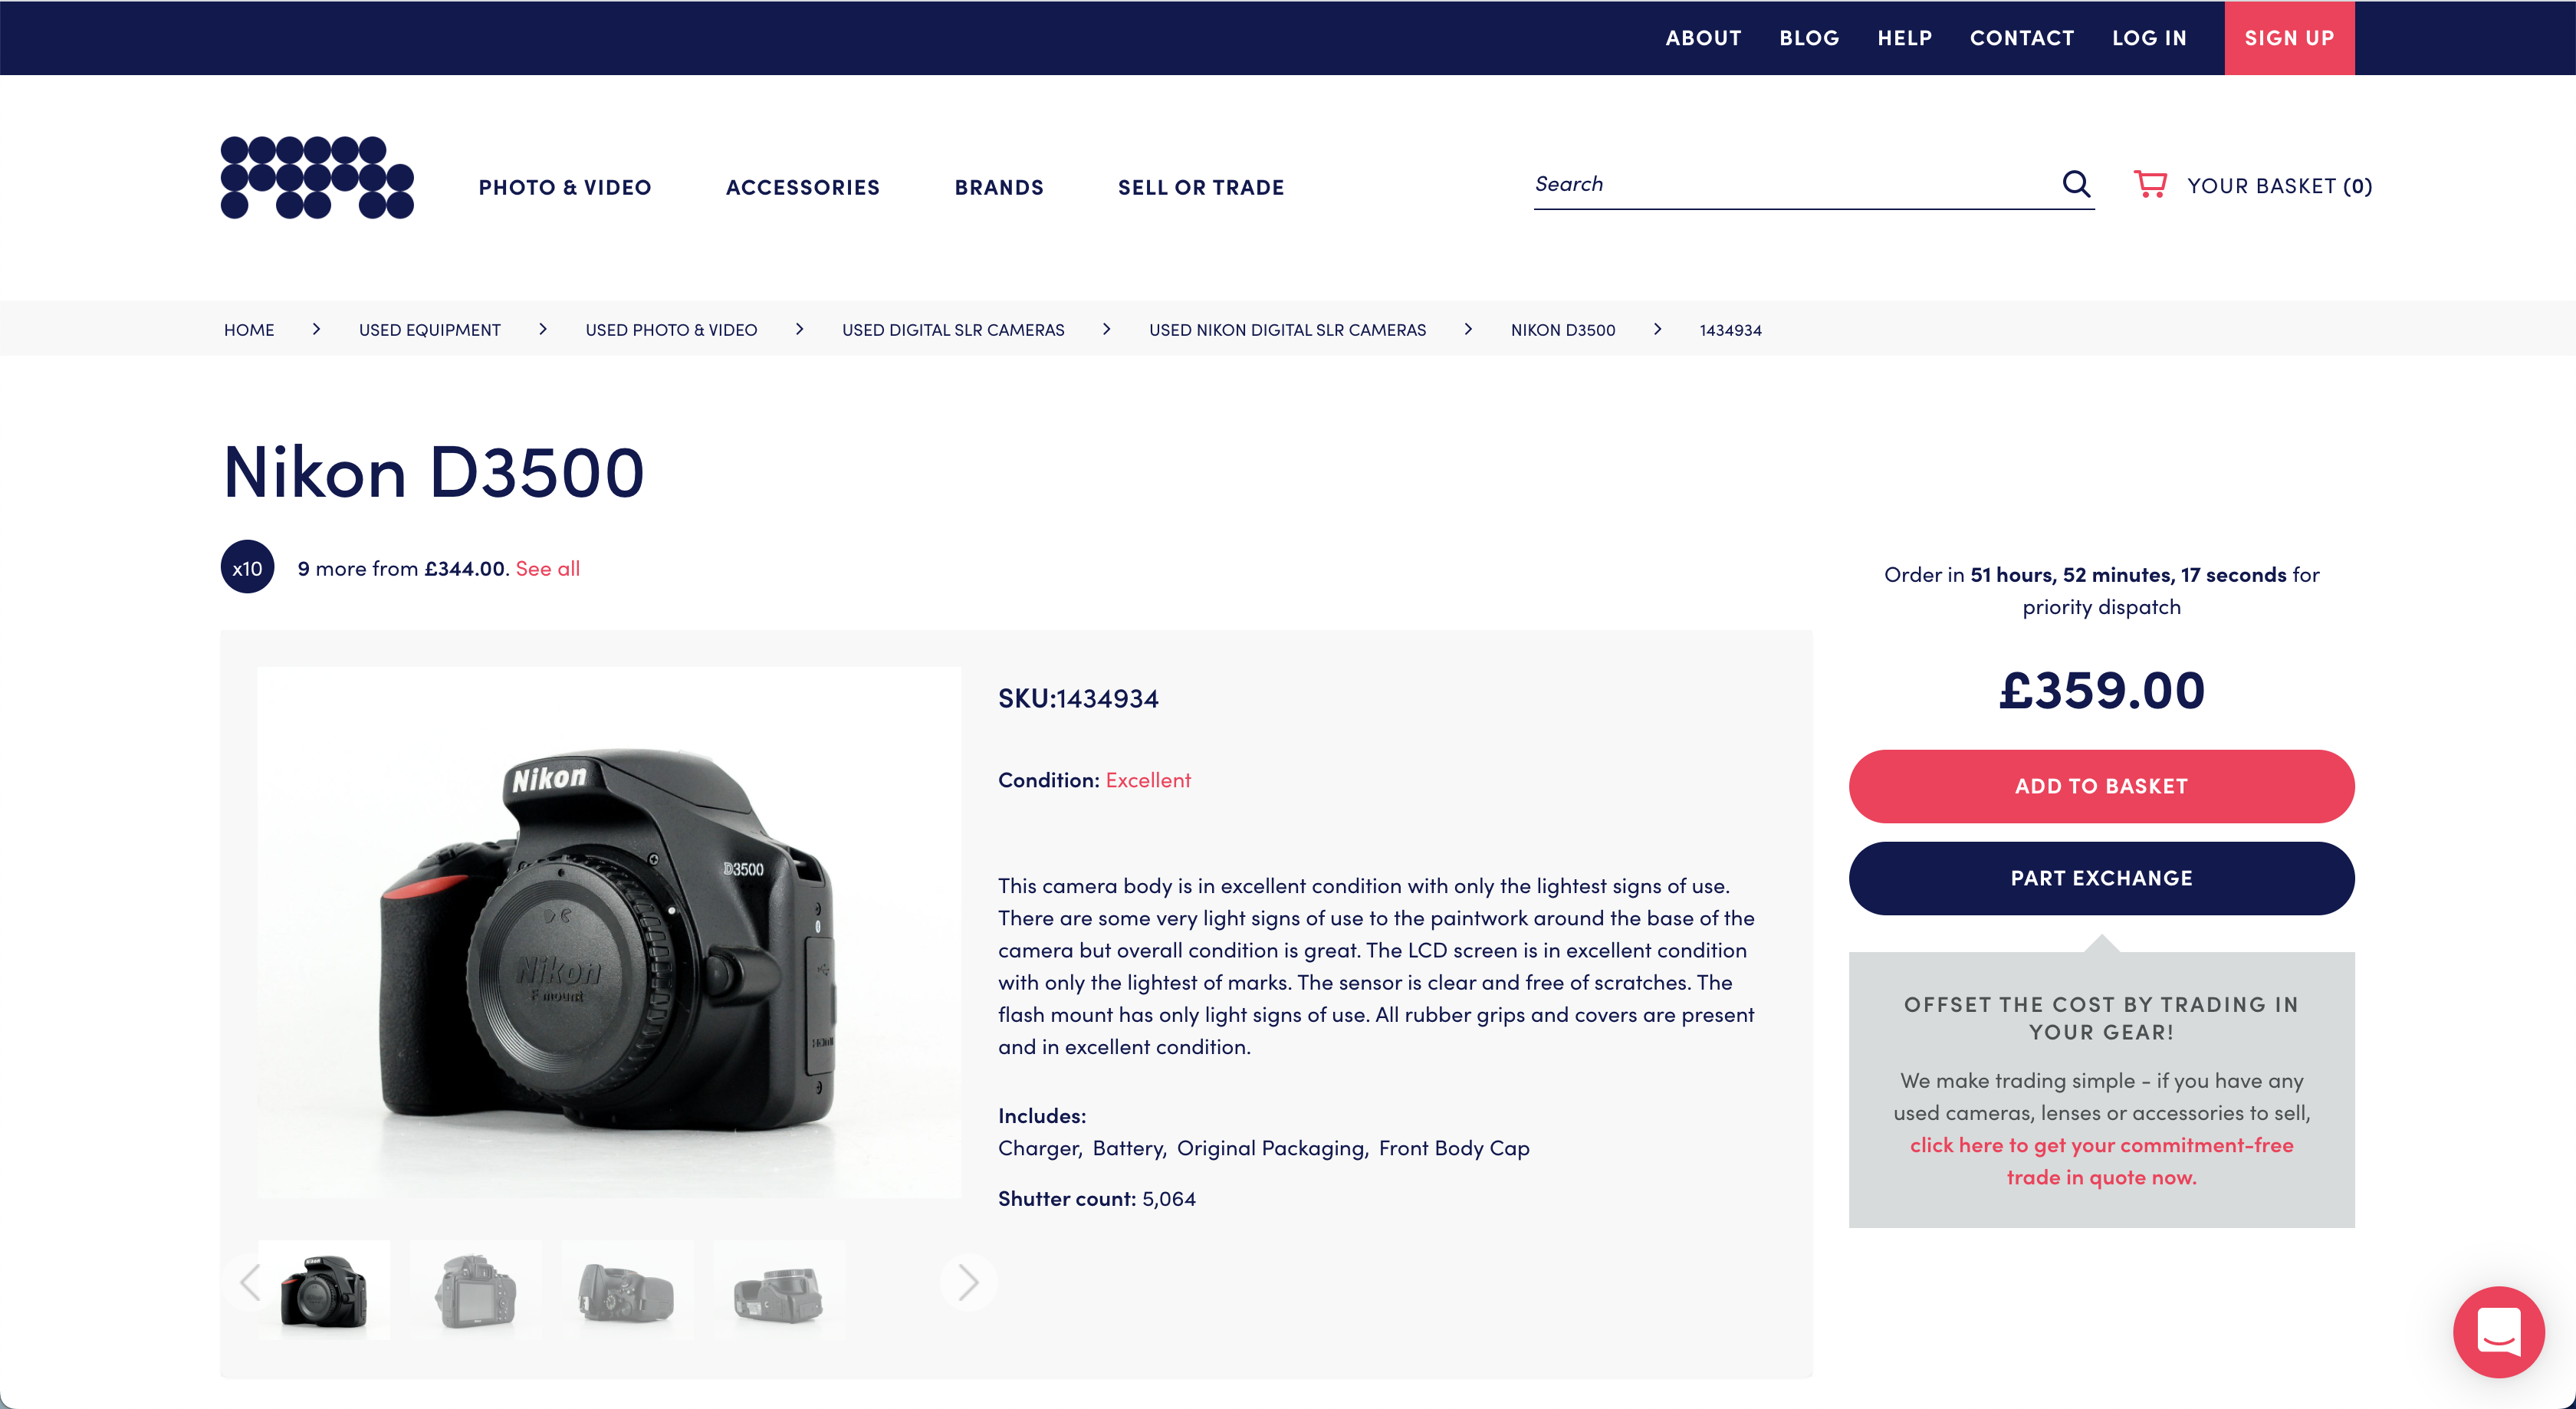
\includegraphics[scale=0.27]{ch1_analysis/mpb_listing.png}
    \caption{Example listing for a camera on MPB}
    \label{fig:ch1_mpb}
\end{figure}
\subsubsection{Advantages}
One feature that the site does well is that it allows the user to easily see what condition the camera is in. One issue with buying second hand is that people can be vague about what state the gear is in. This alleviates the issue by providing a simple solution that people can understand, this is also standardised across the site. Another advantage is that all the listings for a particular camera are in the same place, the user can search for a camera, say ‘D3500’ and see all the listings for that model. This makes finding the specific camera to buy much easier.
\subsubsection{Disadvantages}
One disadvantage of the site is that it doesn’t attach a user to the individual listing. This means that a buyer that is unsure in what they are buying doesn’t have an easy point of contact should they want to query the on the product. This means that should they be unsure they will have to go through a commercial help solution that doesn’t provide a personal experience to the user.
\subsubsection{Features to include}
One item that MPB does well is that it provides the items that a user will get along with the camera body, this would be a good section to include within the project as it would enable people to get a proper idea of what they are buying and what they might have to invest in separately.

\subsection{Existing solution: London Camera Exchange \parencite{lcegroup}}
London Camera Exchange provides a marketplace for both new and second-hand gear. The site is the counterpart to the in-person shops that London Camera Exchange have. The company sell products for both digital and film photography along with other imaging kit such as binoculars or telescopes.
\begin{figure}[H]
    \centering
    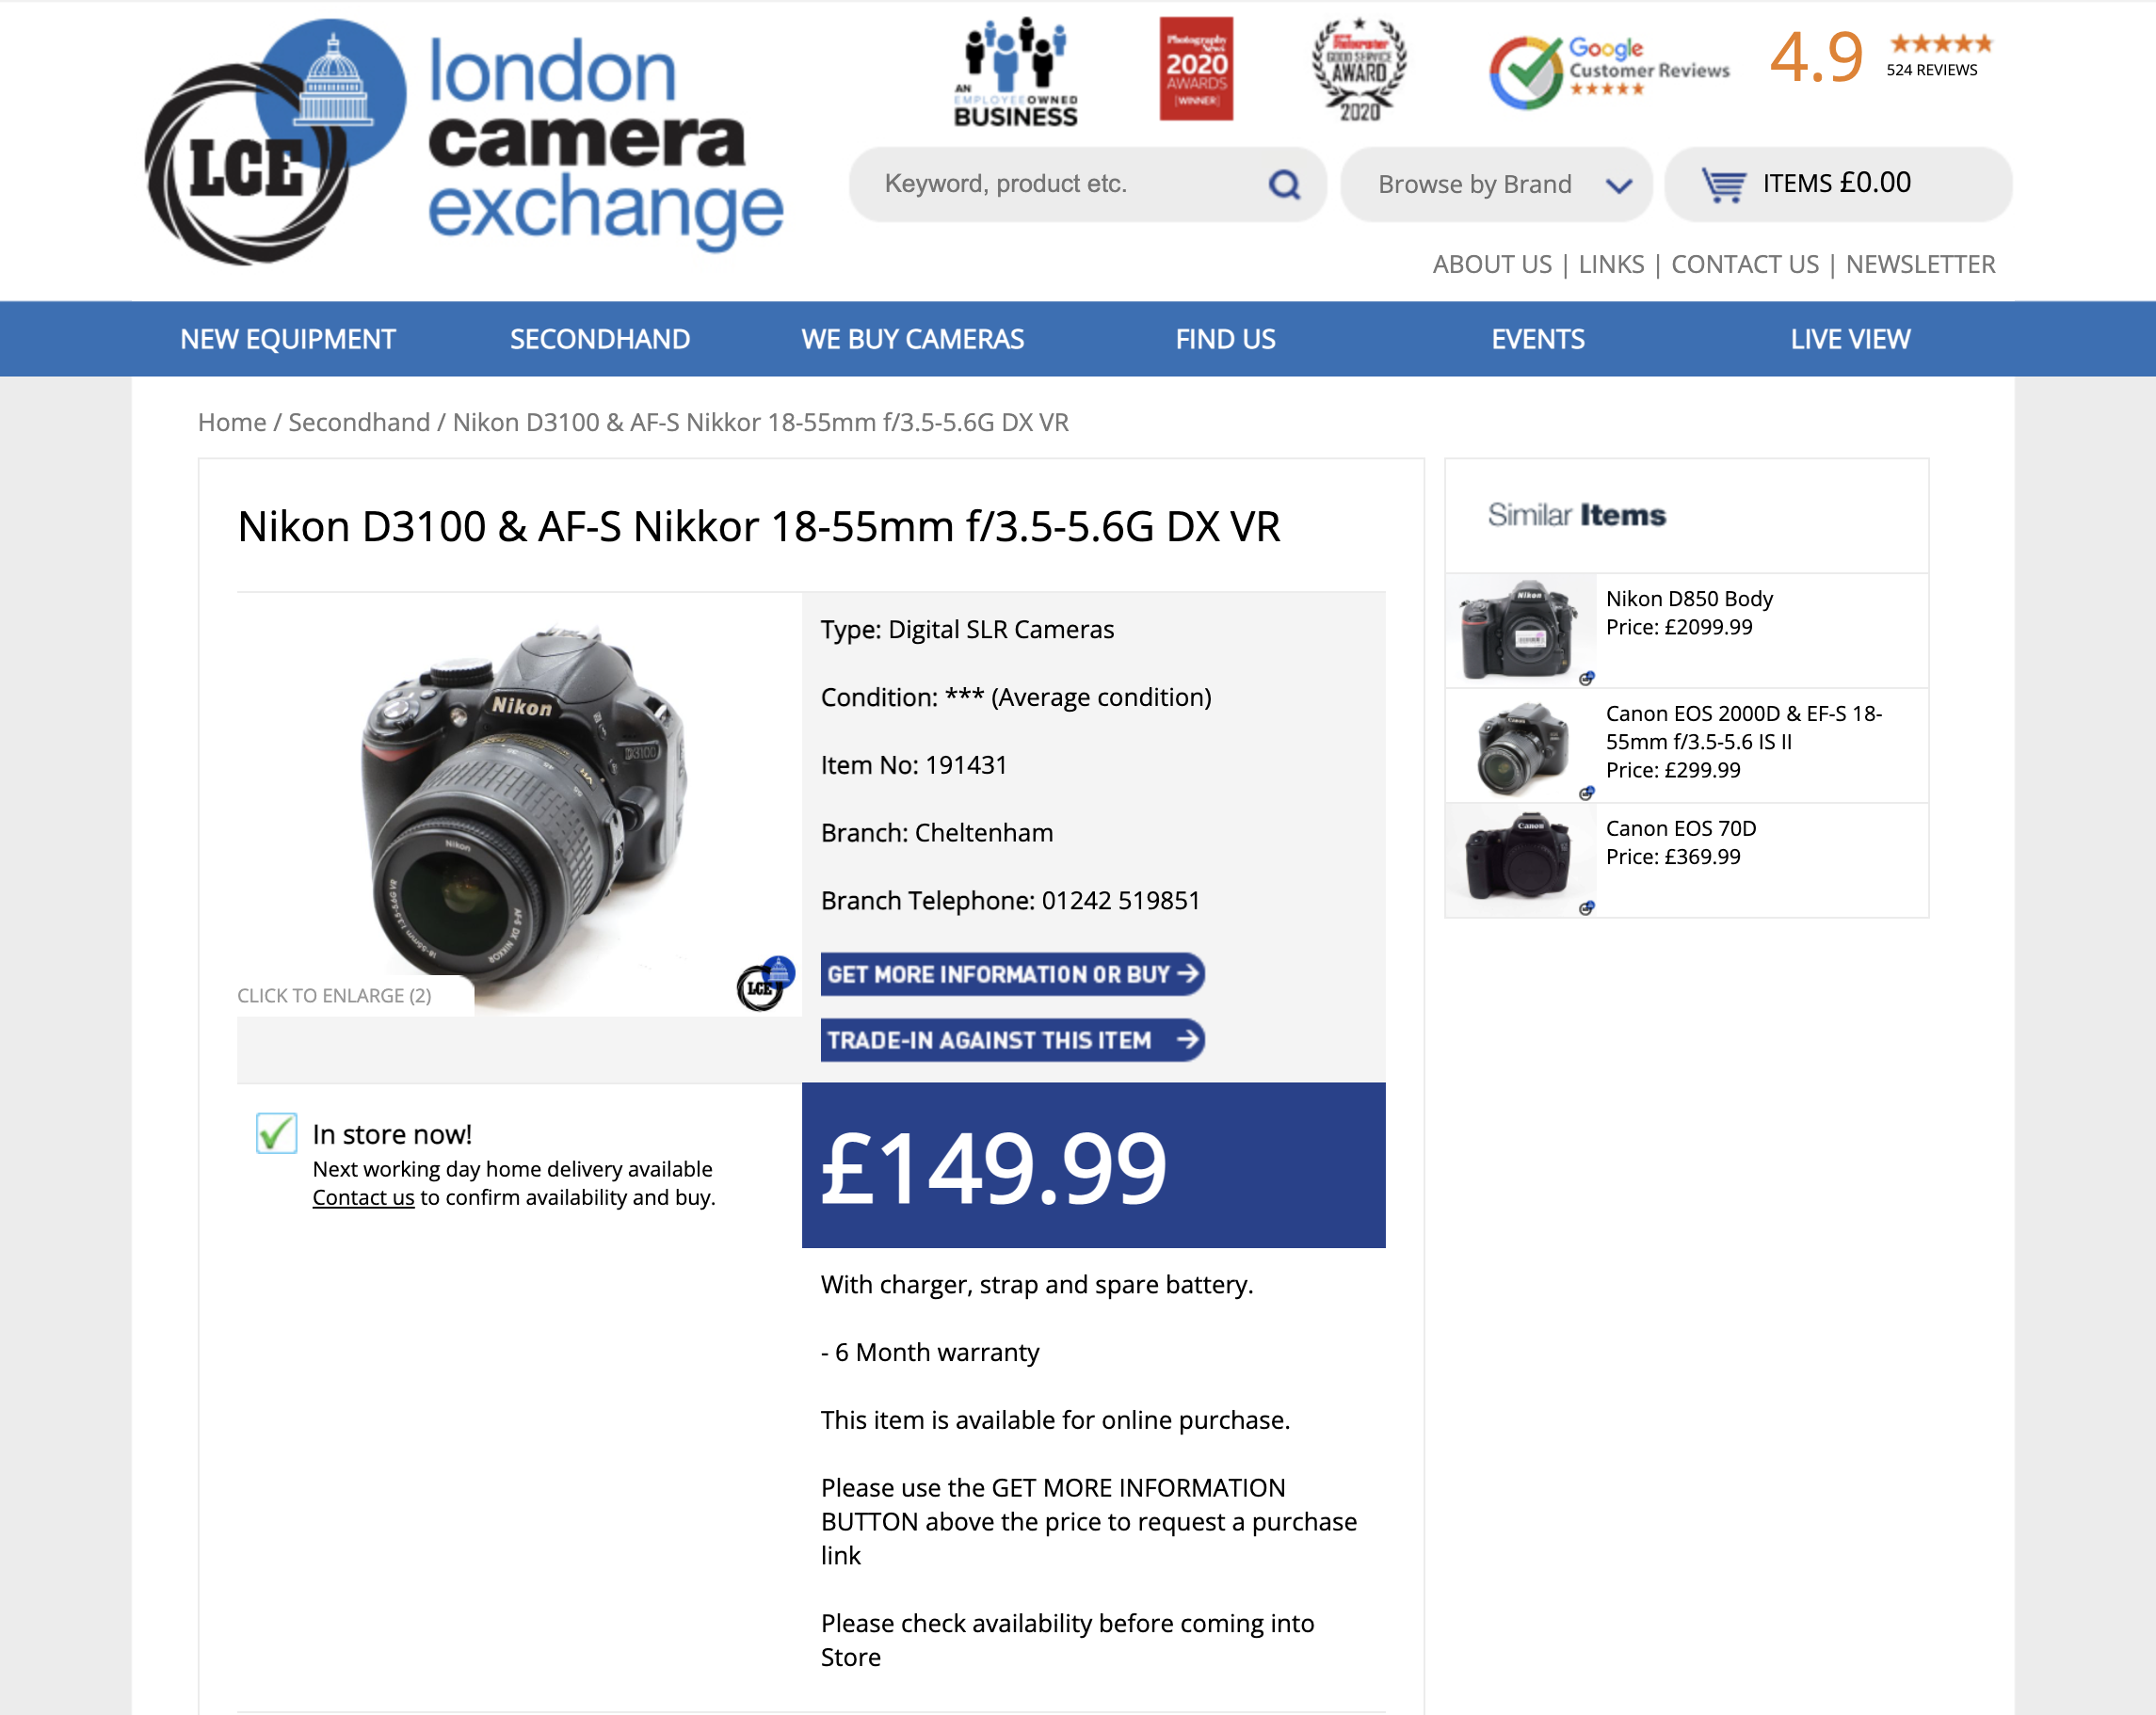
\includegraphics[scale=0.27]{ch1_analysis/lce_listing.png}
    \caption{Example listing for a second-hand camera on the London Camera Exchange}
    \label{fig:ch1_lce}
\end{figure}
\subsubsection{Advantages}
One advantage is that London Camera Exchange allows the user to see the quality of the camera that they are buying. This is rated from 1-5 stars by the company when the camera is sent in, and the levels are standardised across the various branches. This means that the user will always know what quality the product will be should they choose to buy the item. Another advantage is that the site lists what accessories will come with the camera when it is purchased. This makes choosing which specific camera to buy easier. Another advantage is the site also sells photography gear aside from cameras and lenses which makes it easier for a user to get everything they might need for photography from one place.
\subsubsection{Disadvantages}
One disadvantage of the site is that there is no easy buy button to press if the user would like to purchase an item. Instead, the user is given an email for the store and must wait for a person in the shop to confirm the item is still available and to receive an email back with a link to purchase the item. This is not good for the site as it makes it difficult for users to buy items and encourages them to look for easier solutions should they want to purchase an item. This however does only apply for second hand purchases. The website is also crowded leading to it being hard to navigate and find what you want as a first time user.
\subsubsection{Features to include}
For my project, I want to include the features of a quality rating and the selling of other photography gear. The quality rating from the London Camera Exchange works well to allow anyone to see what quality the camera gear is in and so makes the experience better for anyone who is looking at equipment. By allowing the listing of other photography gear, it provides a better experience for the user as they don’t have to hunt around on other websites for the accessories they might also want.

\section{Interviews}
\subsection{Stakeholder 1: Someone selling their camera for the first time, John Smith}
\begin{enumerate}
\item \textbf{How long have you been doing photography?} \\
“I’ve been doing photography for the past 3 years starting with my phone and then later with a family members camera”
\item \textbf{Why did you decide to upgrade to the family camera from the phone?} \\
“I decided to upgrade to a camera when I felt that the phone was limiting me in what photos I wanted to take. The new family camera wasn’t a solution to every problem such as I couldn’t take RAW photos still, but I could at least zoom in and out and take better low-light photos”
\item \textbf{What made you decide to buy your own camera?} \\
“I’ve really enjoyed doing photography with my family camera however it is only a basic compact system that doesn’t allow for changing lenses or for using lower apertures”
\item \textbf{Why do you look for in your new camera?} \\
“I ideally want a camera that I can use for a long while and not have to upgrade again soon. I also want something that I can change the lens on so that I can take different styles of photos. A camera that could shoot RAW images would be really good and would allow me to better develop me editing as well.”
\item \textbf{How long have you been looking for a camera to upgrade too?} \\
“I have been looking for around 3 months now. I’ve been researching various websites in order to try and work out what I should get”
\item \textbf{Why have you been looking for so long?} \\
“It has been really difficult to find what I’m after, there seems to be so much conflicting information on what is available, modern and actually worth buying. It’s also difficult to find the right place to buy from.”
\item \textbf{You’ve mentioned you struggle to find the right place to buy from, what issues have you had?} \\
“I can’t seem to find the right website, every page I’ve looked at seems to have a downfall. The actual manufactures website doesn’t stock the product as I’m often looking at older gear. If I go to Amazon, the listing seems too expensive as if its listed still at new price. I’ve tried to use an auction website such as eBay but I’m struggling with the individual listings.”
\item \textbf{What has been the issue with eBay listings?} \\
“With eBay, the quality of each listing seems to change so drastically. I might find a listing for the product I like at a good price, but I can’t find any information on the quality of the item. Alternatively, a similar product may pop up, but I don’t have any knowledge on that model and so can’t decide if it is good for me”
\item \textbf{What would an ideal listing look like for you?} \\
“An ideal listing would be one with lots of images from all angels of the camera so that I can see what the condition is like. If I’m also able to see what else will be included when I buy the product that would be useful. If the listing also contained information on the cameras information that is always useful but rarely done.”
\item \textbf{I’m proposing that with each listing the buyer will be able to see a full stats breakdown of the camera, would that be useful?} \\
“Yes, I think so. If attached to every listing, there is an easy stats list then I can more easily compare two cameras I’m viewing”
\end{enumerate}

\subsection{Stakeholder 2: Someone looking to buy a camera for specific needs, Phil Martin}
\begin{enumerate}
\item \textbf{What do you currently do with photography?} \\
“I commercially shoot weddings right now for people and then do freelance work in-between for what people need”
\item \textbf{What does your current gear look like?} \\
“I currently use two large DSLR bodies and a host of lenses to cover all needs I may have when working. As part of the job, I also carry around a collection of other accessories such as filters, spare batteries and memory cards.”
\item \textbf{Your current working gear sounds good, why do you want to upgrade?} \\
“The cameras are starting to become old and have a large shutter count on them meaning they might break soon. The technology has also evolved, and I want to switch to mirrorless system.”
\item \textbf{Where have you looked so far?} \\
“I’ve looked mainly at second-hand sites, prices for new camera bodies and lenses are still too high for what I can afford at this time. I’ve mainly looked at eBay but also local selling sites such as Facebook Marketplace.”
\item \textbf{What has the experience been like?} \\
“The experience has been a mixed bag, on the one hand there is lots of options out there at good prices however the amount of information on each of the listings seem to vary drastically. In some its lots of information on what the quality of the camera is like and how it has been used yet on others there isn’t anything more than a few words.”
\item \textbf{Would you find it useful to have a quality rating on each of the listings which meant you could easily see what condition the camera was in?} \\
“I think that would be useful for me as I would be able to avoid the listings for broken cameras or those which have already had a lot of use since I need newer gear that can be used every day.”
\item \textbf{What do you plan to do with your old gear?} \\
“In the short them I will likely hold onto my old equipment in case I can’t adapt to the new gear. In the long run however, I think that I would like to sell the gear so that I can recoup some of the money spent on the newer mirrorless cameras.”
\item \textbf{Do you struggle with anything when it comes to selling second hand gear?} \\
“I find it tough to know how I should be pricing the item, on the one hand, I’m able to price gear that’s still in good condition but when it comes to selling my two main cameras, they have been used so much it’s difficult to know”
\item \textbf{Would a price recommendation help when it comes to selling?} \\
“I think it would however I worry that it won’t be accurate for gear that is in bad condition. I don’t want to have to be confined to a single price point if I want to sell”
\end{enumerate}

\section{Features of proposed solution}
\subsection{User login system}
The site will have the ability for users to sign up and then later log back in. This will be a required factor to access the site and to be able to bid on items. This will work through having the user enter their details, verifying them before adding them to the database. When signing in the user will only have to enter their username and password which will allow them to log into the program.  
\subsection{Search box}
The website will have a search box that allows buyers to search for listings for a camera that they might want to buy. The query will be sent to a database and the relevant results will be sent back in the form of a table where the user will be allowed to
\subsection{Price recommendation}
When the user comes to sell their gear, they will be able to enter the make and model of their camera and it will return the average price of previously sold items. This will be based off the previously sold items on the site for the camera. This will support and help people who are new to selling camera gear.
\subsection{Camera information on the listing}
Using a database of cameras and their corresponding information, each listing will contain a table of the stats of the camera that is listed. This will be achieved through the user adding what camera they are selling as a requirement for the listing. This information can then be used to show the information for the camera allowing for easier comparison.
\subsection{Similar listings shown below the main listing}
Below the listing that the user is viewing, similar listings of the same camera will be shown. This will allow the user to see other options when it comes to buying. This will enable users to browse other listings of the same camera that might be better quality or might contain more products.
\subsection{Limitations of the proposed solution}
One limitation of the system is that the price recommendation will require a substantial amount of sold listings in order to best work. The number of listings needed are unrealistic for the project which will mean that the price recommendation might not be the most accurate that it can be. 
Another limitation for the project is that not every camera can be included in the information section. This is due to the vast number of cameras that there are in the world and so it will be unrealistic for every detail of every camera to be known. 

\section{Hardware and software requirements}
\subsection{Development requirements}
From a hardware perspective, the program will be written on a laptop comprising of an Intel i5 CPU with Iris Plus 645 graphics. The laptop also has 8GB of ram and 128GB of storage space. The program will be written in the Visual Studio Code IDE \parencite{visualstudio}.For the SQL required in the project, MySQL \parencite{mysql} will be used and hosted on a Raspberry Pi which has a Quad core Cortex-A72 CPU and 4gb of ram \parencite{raspberry_pi}. The SQL database will be accessed remotely through the MySQLWorkbench \parencite{mysql_workbench} software. The PHP website will also be hosted on the Raspberry Pi throughout development. To allow access to the Raspberry Pi outside of my home network, I will be creating a virtual private network (VPN) through the OpenVPN system \parencite{openvpn}. 

\subsection{Project requirements}
In order to run the project, the user will require an internet connection alongside a web-browser in order to access the website such as Google Chrome \parencite{google}, Safari \parencite{apple}. The machine must be able to have the facilities for client-side processing as this is required for some aspects of the site. Whilst machine specifications are unlikely to be an issue for a website, the user should ideally have at least an Intel Pentium and 2gb of ram. Integrated graphics will suffice for this project due to the low intensity. Due to the program being hosted on the internet, the only amount of space required on the hard-disk is that required to hold the web-browser. 

\section{Success Criteria \parencite{oquinn}}
\begin{center}
\begin{longtable}{|p{12.5cm}|p{15mm}|}
  \hline
  \textbf{Criteria} & \textbf{Met?} \\
  \hline
  \endfirsthead
  \hline
  \textbf{Criteria} & \textbf{Met?} \\
  \hline
  \endhead
  \hline 

  \endfoot
  \endlastfoot
  
    The user should be able to enter an email, username, password and card details in a form on the sign-up page & ~ \\ \hline
    The user should have the data verified against the database and if unique they are allowed to continue to the site else, they are sent back to the landing page with an error & ~ \\ \hline
    A returning user should be able to log back into the page through a form where they can enter their username and password & ~ \\ \hline
    The details that the user has entered should be checked to see if the password matches the corresponding username and if so, the user is allowed to continue to the site & ~ \\ \hline
    If the details do not match, the user should be sent back to the landing page with an error & ~ \\ \hline
    The user will have two buttons on the home page that allows them to click either search listings or to create a listing & ~ \\ \hline
    Should the user choose to search they should be able to type the camera they want to search for into a search box & ~ \\ \hline
    The camera that the user entered into the search box form is used as the search term for a query of the database table & ~ \\ \hline
    The results of the query for the camera are then displayed to the user in the form of the table. The table will show the current price of the item along with a brief description with the user being able to click on the camera that they want to view the full listing of & ~ \\ \hline
    The name of the camera is used as a query term for the camera information table in the database & ~ \\ \hline
    All the information on the camera is retrieved using the query and the information on a camera is displayed in a table on the listing page & ~ \\ \hline
    The user can enter a bid for the item using a box on the page. If the bid is higher, then the bid is added to the table along with the user’s username and email. If not the highest bid an error is returned & ~ \\ \hline
    Both the winner and the seller are contacted when the listing ends. The winner is told they have won, and how much they paid the lister is told that the item has sold and at what price it has sold for. & ~ \\ \hline
    When the listing has finished it is removed from the current listings and moved to the sold listings & ~ \\ \hline
    Once a listing is sold, use the sold camera as a search term to gather all the sold listing prices of a camera & ~ \\ \hline
    Store all the values of the sold listings for a particular camera in an array & ~ \\ \hline
    A program will take the array and create a mean value out of the values which is the written to the database table & ~ \\ \hline
    On the home page the user also has the option of pressing the create a listing button which will take them to the page to create a new listing for the site & ~ \\ \hline
    On the create a listing page the user is given a form that has boxes for camera, description, quality, how long they want a listing to last, starting bid with all the information being written to a database table and given a listing id & ~ \\ \hline
    The user is able to upload pictures of the camera to the site with these being stored in a database attached to the listing id & ~ \\ \hline
    Once the user has finished the entire listing form, they can press a button and have the listing added to the current listings database & ~ \\ \hline
    Once the user has completed their listing, they are sent back to the homepage & ~ \\ \hline
    Once the user has finished, they are able to sign out of their account which will return then back to the landing page of the site & ~ \\ \hline
    \caption{Success criteria for the project}
\label{tab:success_criteria}
\end{longtable}
\end{center}